Since we now have the AIOE and complementarity scores, let us explore the data by looking at the labor supply and demand.

\subsection{Defining the 2-by-2 Framework}
We classified each job in the MCA dataset using its AI Occupational Exposure (AIOE) 
and complementarity scores. Jobs with below-median AIOE were categorized as 
\textit{Low Exposure}, while those with above-median AIOE were considered 
\textit{High Exposure}. Within each exposure group, jobs were further subdivided 
based on whether their complementarity score fell below or above the overall median. 

This framework produces four job types. Low-exposure jobs are either 
\textit{Protected} (high complementarity) or \textit{Isolated} (low complementarity). 
High-exposure jobs are either \textit{Augmentable} (high complementarity) or 
\textit{Automatable} (low complementarity). This is summarized in Figure~\ref{fig:framework}

\begin{figure}[ht] 
    \centering 
    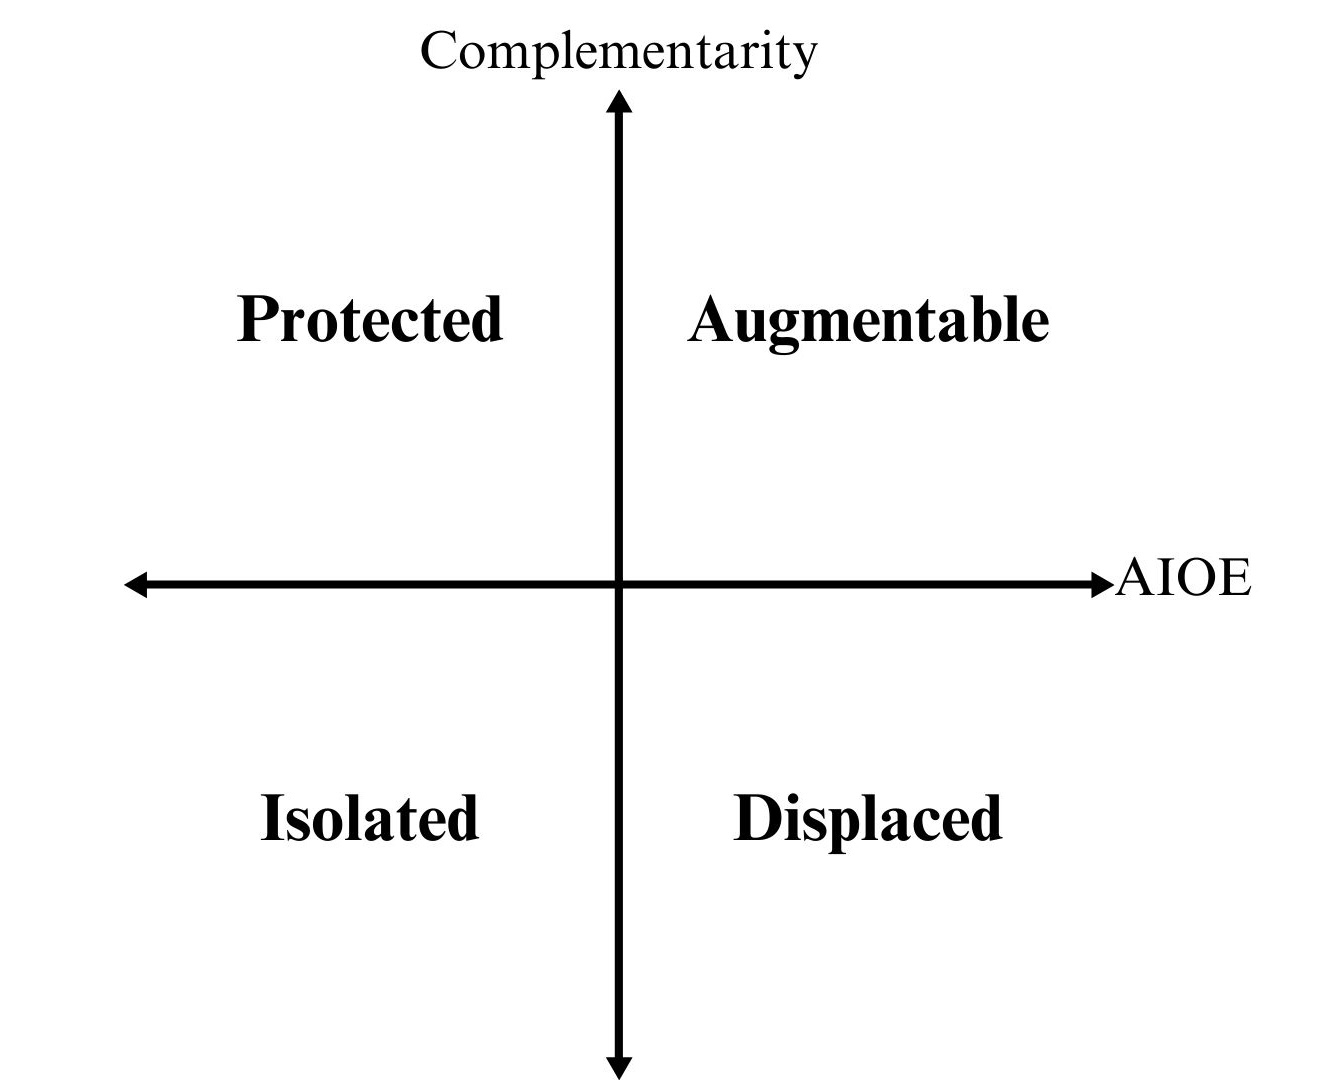
\includegraphics[width=\linewidth]{../figures/framework.jpg} 
    \caption{Matrix of 2-by-2 Framework}
    \label{fig:framework} 
\end{figure}

By organizing the labor market in this way, the challenge shifts from one of job security (whether a job will be replaced) to one of 
skills preparation, emphasizing the need for workers to adapt to AI-intensive tasks.

\subsection{Labor Supply}
From the framework, we can now examine how labor supply differs between workers 
who pursued higher education and those who did not. Table~\ref{tab:ai_exposure_education} 
shows that jobs held by higher-educated workers are disproportionately classified as 
Augmentable, meaning these roles are highly exposed to AI but also benefit 
from strong complementarities. In contrast, jobs held by less-educated workers are 
more likely to fall under the Isolated or Protected categories. 
The former face low complementarity and limited adaptability, while the latter 
remain shielded from AI because of their low exposure.

\begin{table}[h!]
\resizebox{\columnwidth}{!}{%
\begin{tabular}{lcc}
\hline
\textbf{Classification} & \textbf{\makecell{Higher \\ Education}} & \textbf{\makecell{Not Higher \\ Education}} \\
\hline
Augmentable & 75\% & 21\% \\
Protected   & 17\%  & 66\% \\
Isolated    & 3\% & 11\% \\
Displaced   & 4\% & 2\% \\
\hline
\end{tabular}
}
\caption{Percentage of jobs by educational pathway and AI classification.}
\label{tab:ai_exposure_education}
\end{table}

We further visualized this relationship using a scatterplot of AIOE against 
complementarity in Figure~\ref{fig:scatter_aioe_comple}. To illustrate the four classifications, we added representative 
examples of jobs from the MCA dataset. 


\begin{figure}[ht] 
    \centering 
    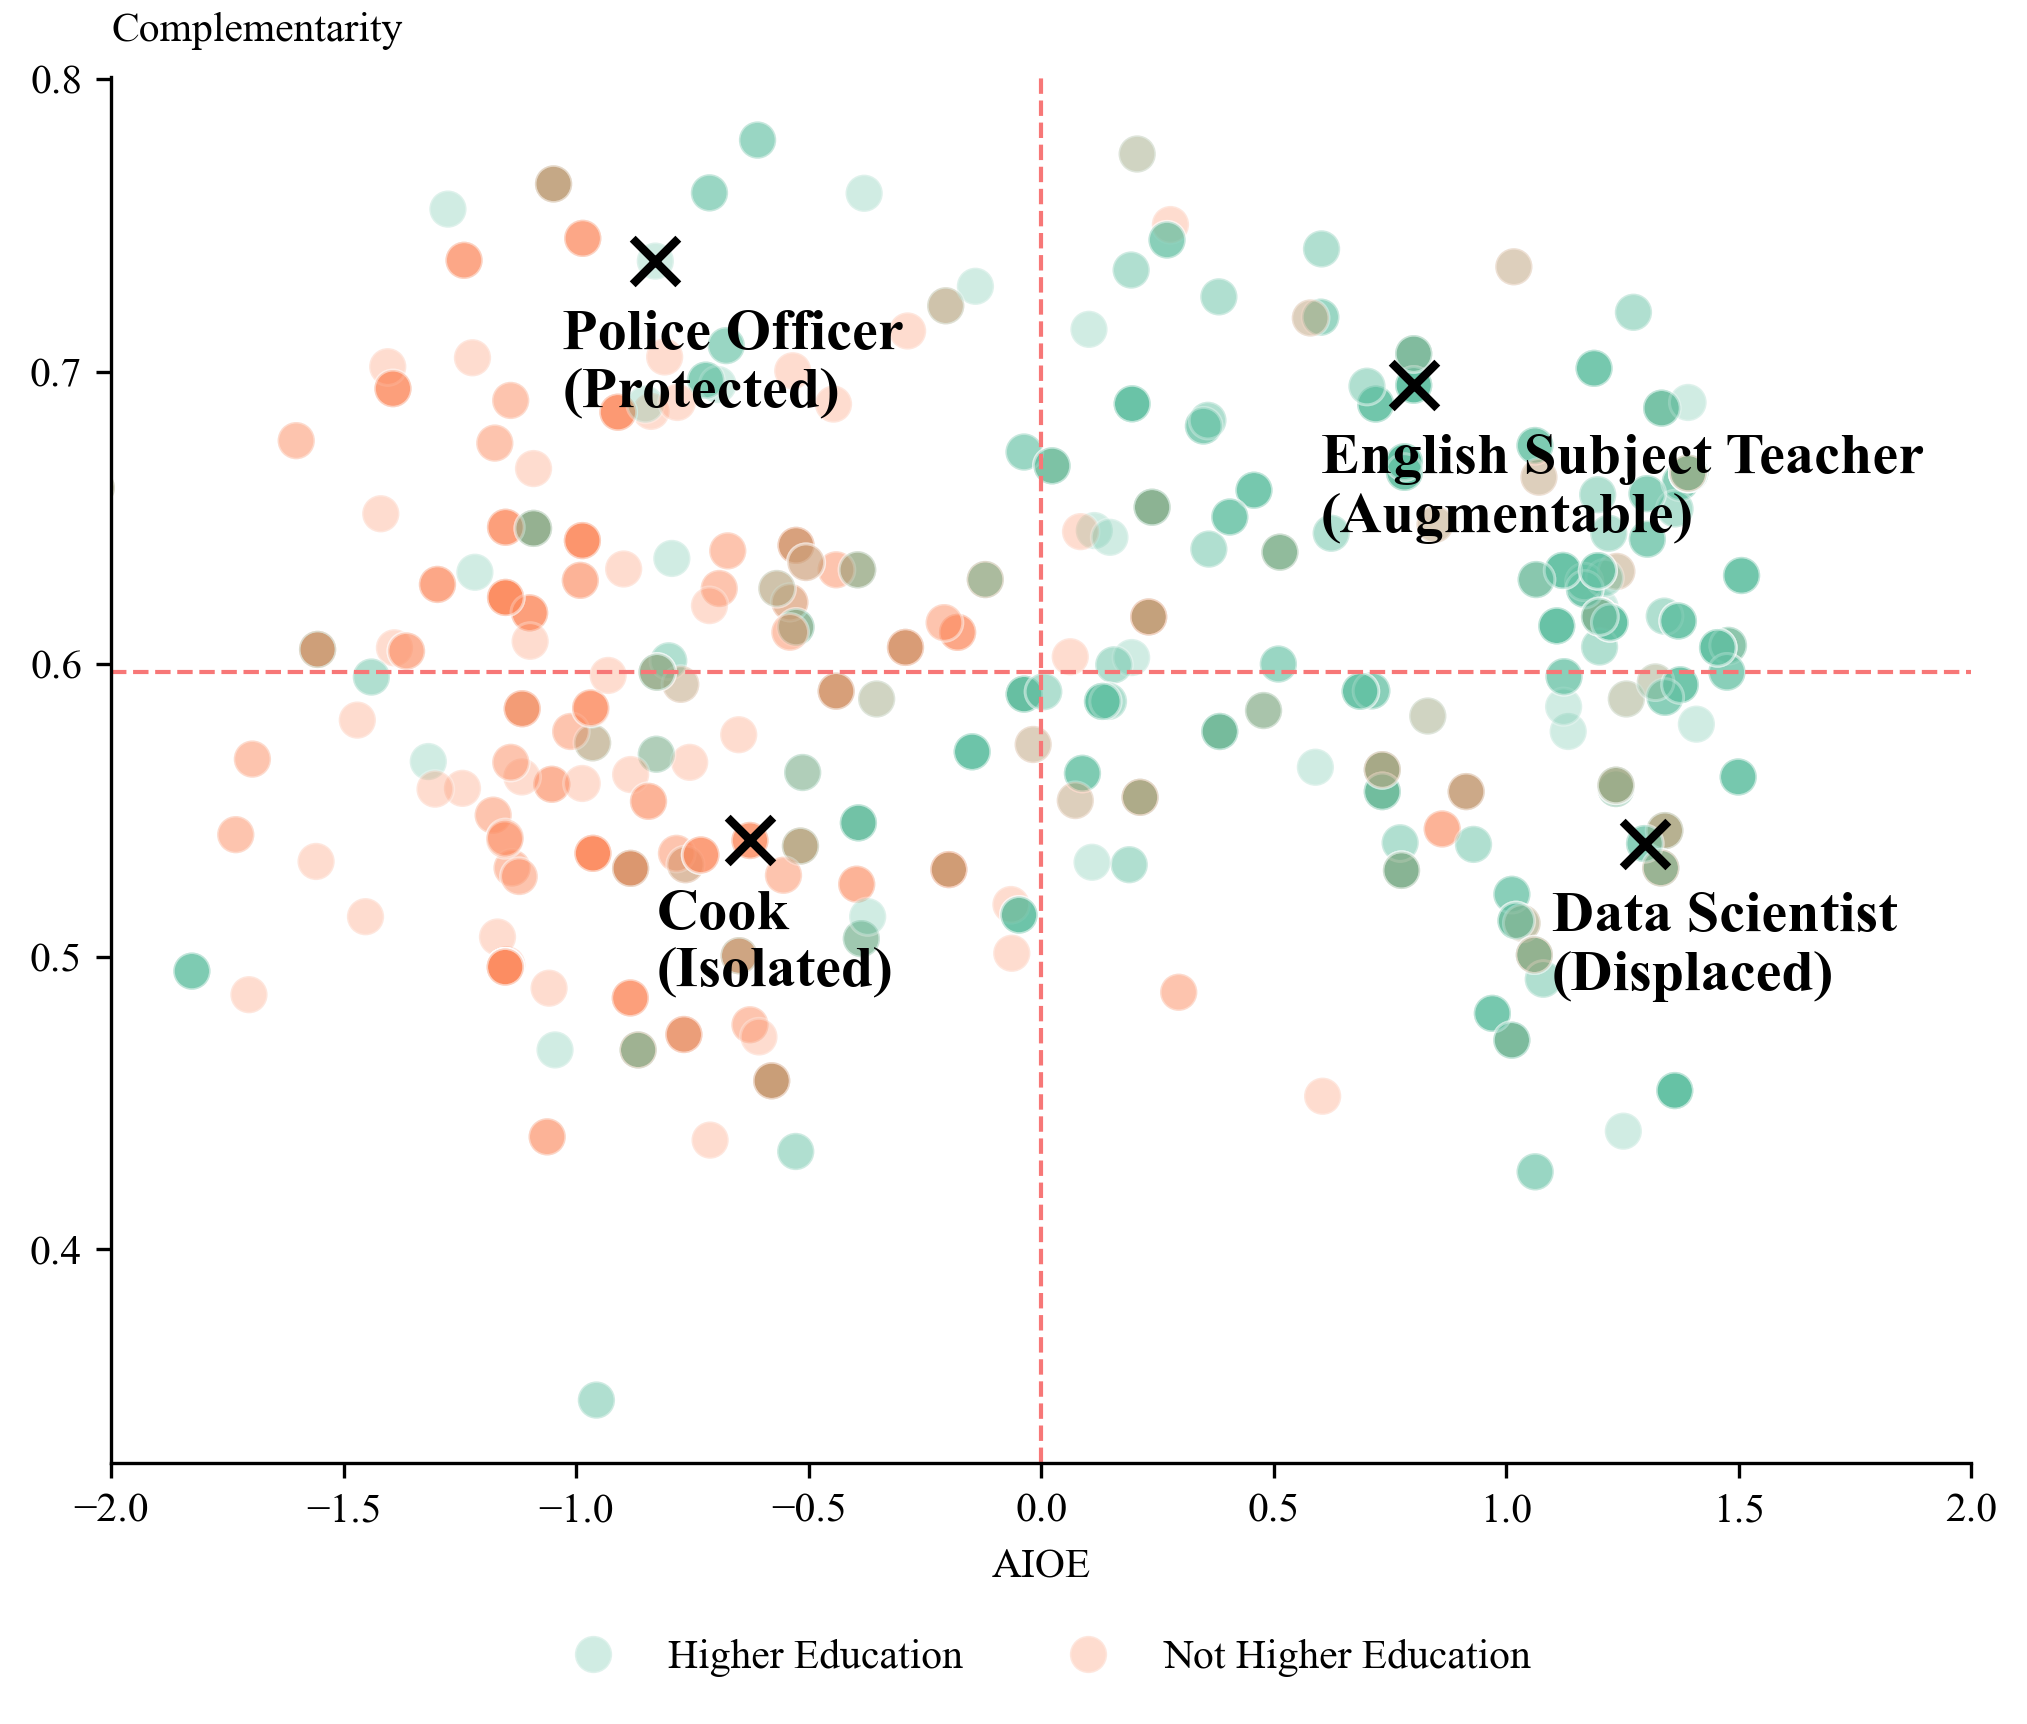
\includegraphics[width=\linewidth]{../figures/aioe_comple.png} 
    \caption{AIOE vs. Complementarity for Filipino Jobs by Educational Pathway}
    \label{fig:scatter_aioe_comple} 
\end{figure}

\subsection{Labor Demand}
To examine labor demand, we used a new metric called the C-AIOE to summarize the risk of replacement at the occupation level to AI.
It is formally defined as:
$$\text{C-AIOE}_i = \text{AIOE}_i \cdot \big(1 - (\theta_i - \theta_{\text{MIN}})\big),$$
where $i$ indexes the job, $\theta_i$ is complementarity to AI, and $\theta_{\text{MIN}}$ is minimum value of $\theta_i$ across all occupations. 
Overall, jobs with higher C-AIOE (because of higher AIOE or lower complementarity) are more likely to face AI replacement. 

This was then aggregated to each of the 21 job sectors by taking the mean C-AIOE of their respective jobs. 
Figure~\ref{fig:sector_caioe} plots the results, highlighting that jobs in financial services, administrative support, 
and ICT have the highest average risk, while construction, agriculture, and manufacturing 
face the lowest.


\begin{figure}[ht] 
    \centering 
    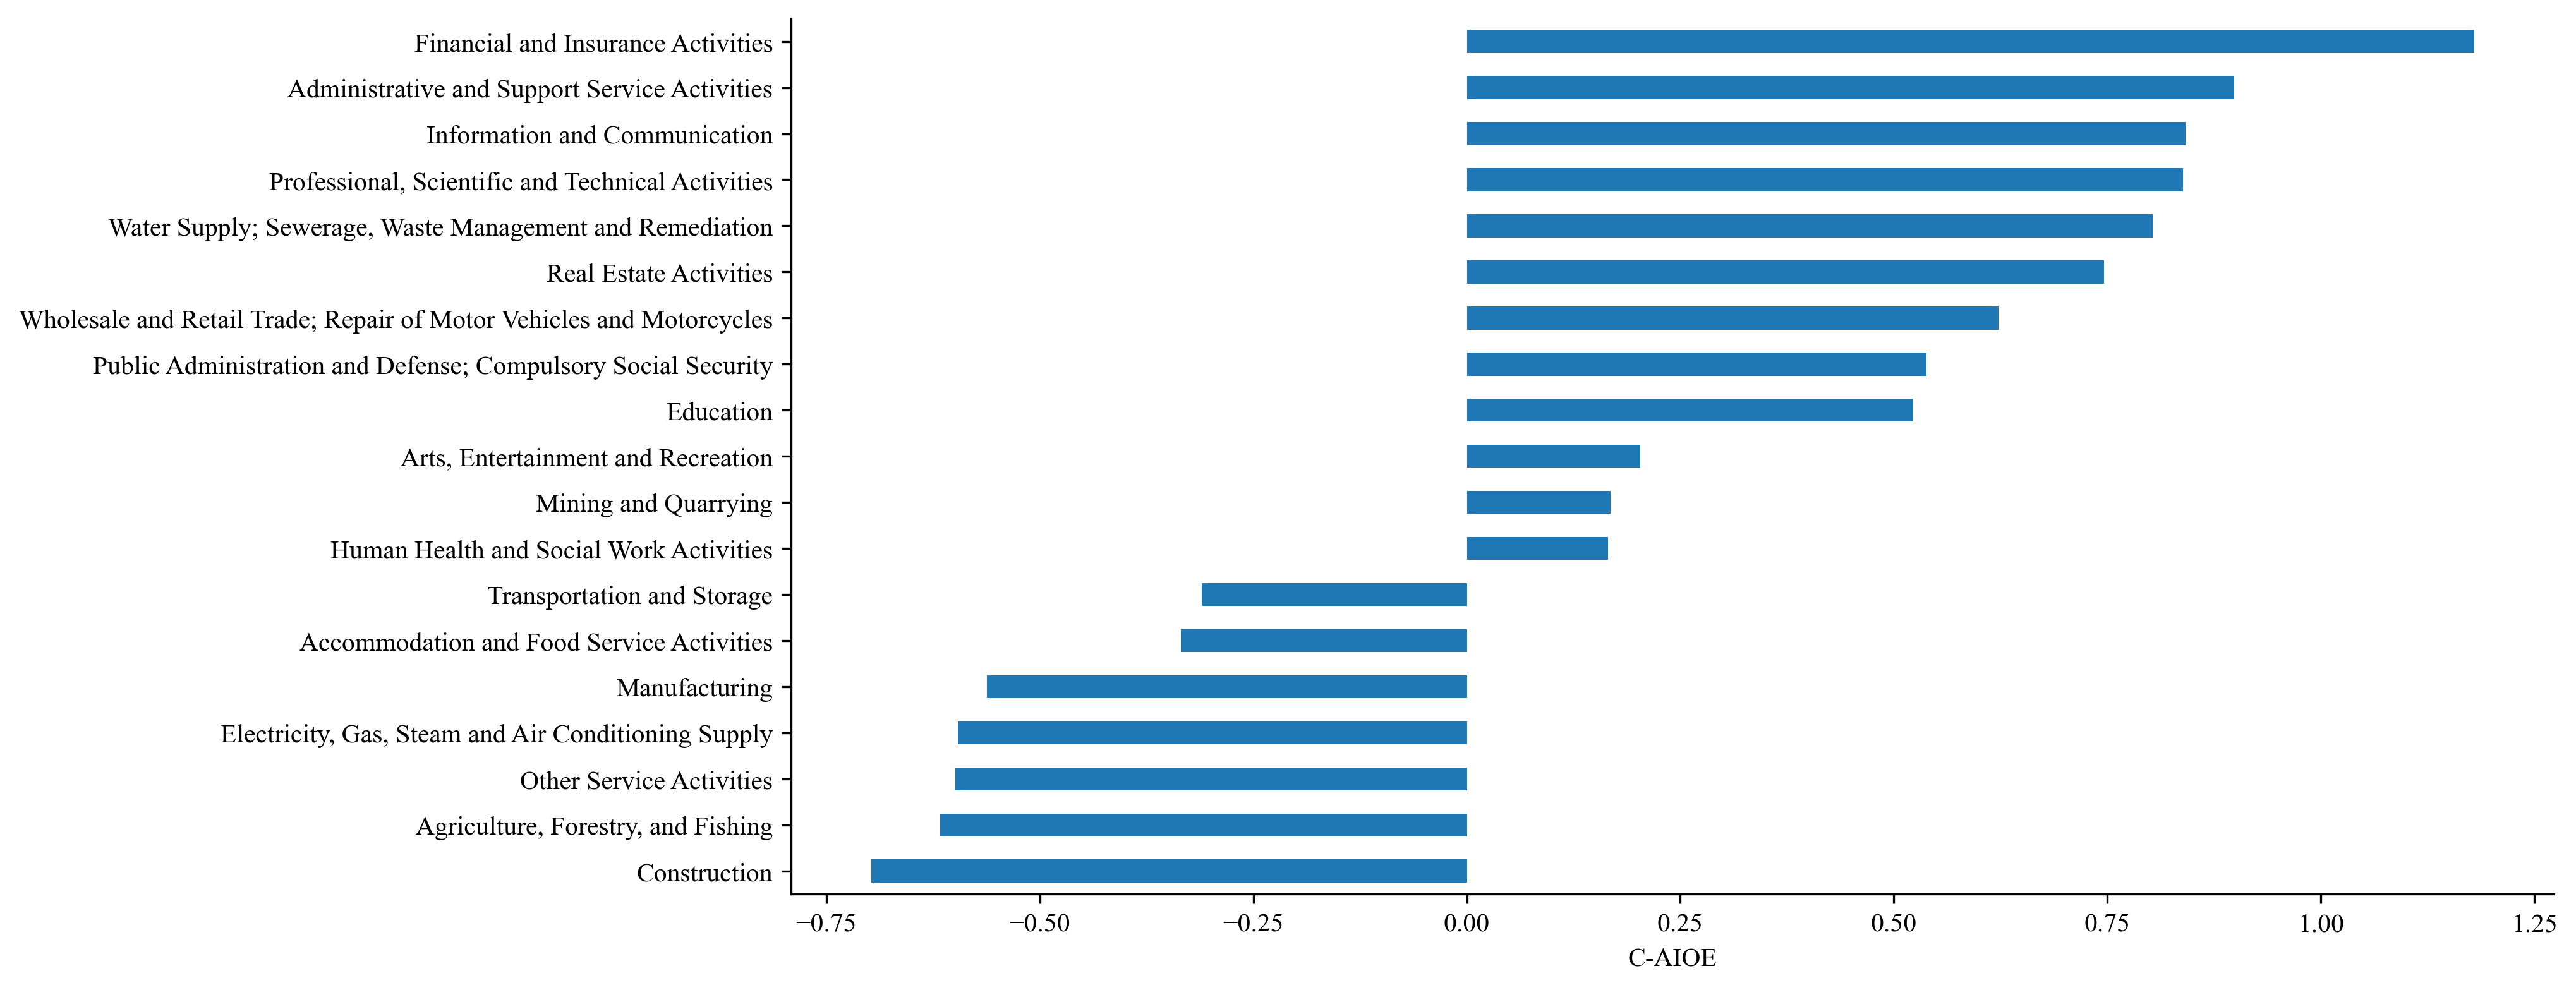
\includegraphics[width=\linewidth]{../figures/sector_caioe.png} 
    \caption{Job Sectors Ranked Most Likely Automated by AI (Based on C-AIOE)}
    \label{fig:sector_caioe} 
\end{figure}

